\placelogofalse
\begin{frame}{Finite Element Method (FEM)?}
\begin{columns}
\column{0.58\linewidth}
\centering
\begin{outline}
  \1 Family of numerical methods
  \2 Solve PDEs
  \2 Mathematical Modelling
  \2 Engineering / Science
  \1 History
  \2 Structural Mechanics in 1940s
  \2 NASTRAN in 1960s
  \2 Widely available now
  \1 Broad and well-funded
\end{outline}

\column{0.38\linewidth}
\centering

\begin{center}
\shadowimage[width=3.5cm]{assets/wiki_car_example.png} 

\shadowimage[width=2.0cm]{assets/fsi.png}
\shadowimage[width=2.0cm]{assets/BLAST_example.png}

\shadowimage[width=3.5cm]{assets/comsol.png}


\end{center}
\end{columns}
\blfootnote{Images from \href{https://en.wikipedia.org/wiki/Finite_element_method}{Wikipedia},
  \href{https://readfast.in/fluid-structure-interaction-in-fea-simulation/}{Readfast},
\href{https://computing.llnl.gov/projects/blast/triple-point-shock-interaction}{LNLL},
\href{https://www.comsol.com}{COMSOL}}
\end{frame}
\placelogotrue

\placelogofalse
\begin{frame}{Geometry and Meshing for FEM}
\begin{columns}
\column{0.58\linewidth}
\centering
\begin{outline}
  \1 FEM requires a discritazation 
  \1 Mesh of volumetric elements
  \1 Bottleneck in production
  \1 Massive research topic
  \1 Meshing Out-of-scope for today 
  \1 Return to meshes later
\end{outline}

\column{0.38\linewidth}
\begin{center}
\centering
%\shadowimage[width=2.5cm]{example_1.png}

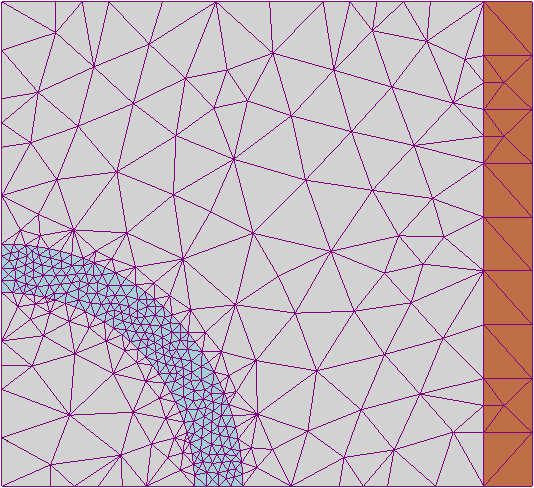
\includegraphics[width=2.8cm]{assets/Example_of_2D_mesh.png}

\vspace{0.2cm}

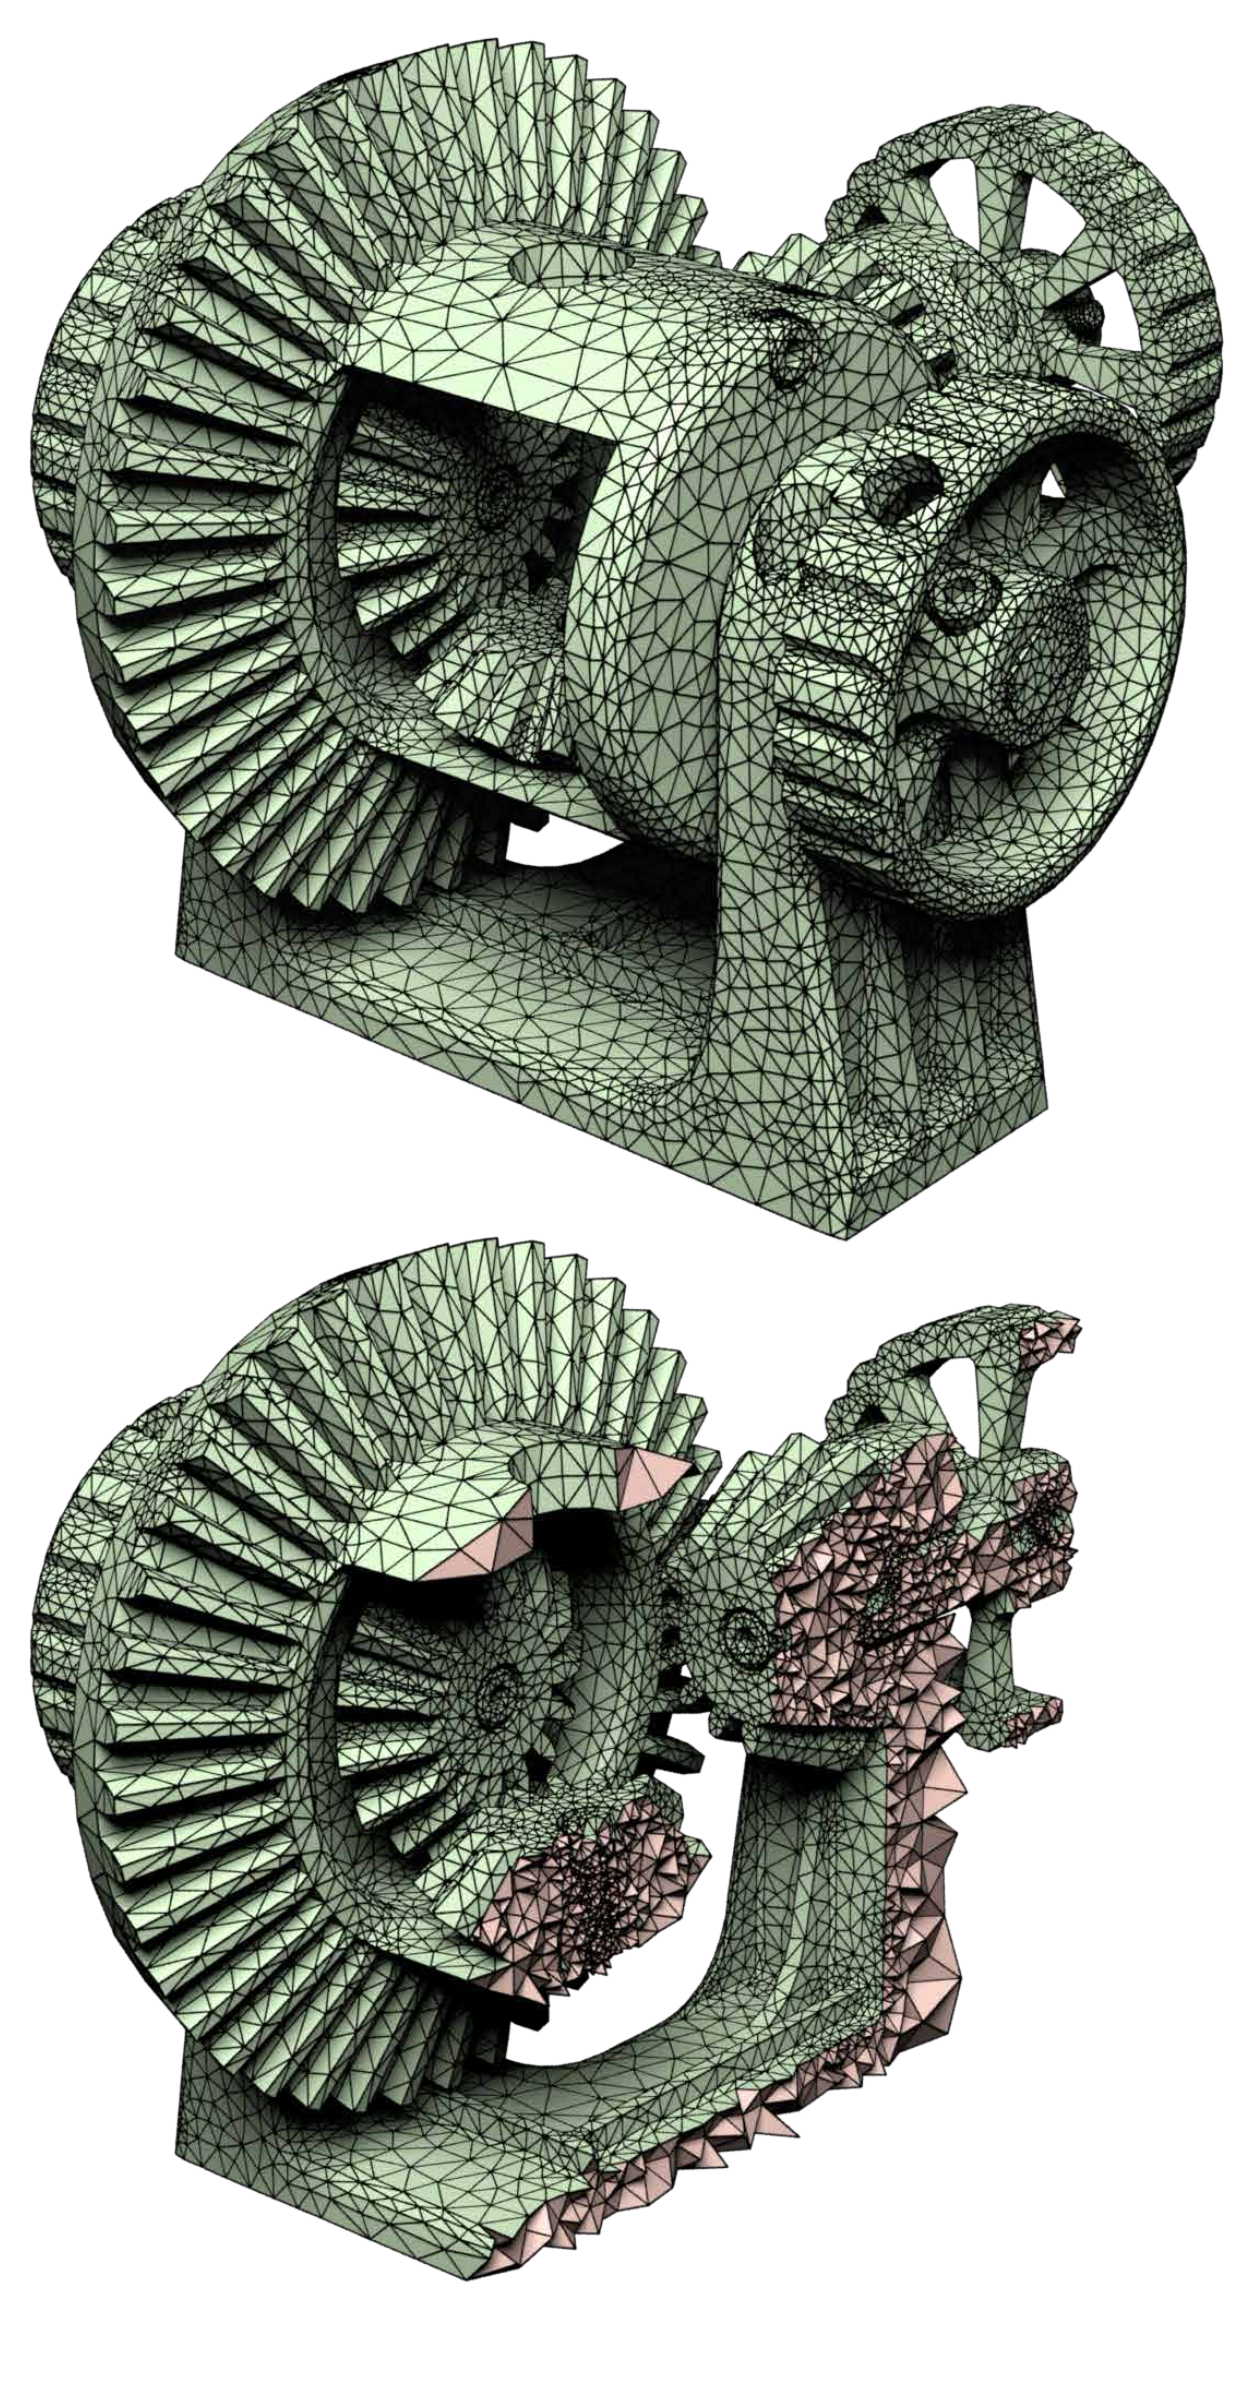
\includegraphics[width=2.5cm]{assets/mesh_example_01.png}


% [trim={left bottom right top},clip]
%
\includegraphics[width=8.5cm, page=3, trim={0 9cm 14cm 0cm},clip]{assets/vec_db_figs.pdf}
\end{center}
\end{columns}
\blfootnote{Images from \href{https://upload.wikimedia.org/wikipedia/commons/8/80/Example_of_2D_mesh.png}{Wikipedia},
\href{https://github.com/wildmeshing/fTetWild}{fTetWild}}
\end{frame}
\placelogotrue

